\chapter{Introducción y Generalidades}

\section{Introducción}
Tipos de arquitecturas de los robots móviles.

\section{Modelos Tradicionales}
Características

Se tiene representación del medio ambiente

\begin{figure}[h!]
	\centering
	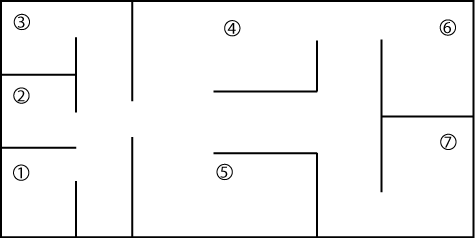
\includegraphics[width=0.5\textwidth]{images/img1.png}
	\captionof{figure}{(Objeto mesa (cuarto 1 $x_{_1}y_{_1},x_{_2}y_{_2},...,x_{_n}y_{_n}$))}
	\label{figura1}
\end{figure}

\paragraph{}
Se planean las acciones y los movimientos del robot.

\begin{wrapfigure}{l}{45 mm}
  \begin{center}
    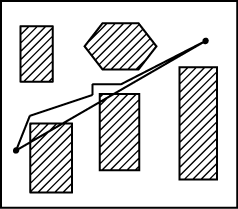
\includegraphics[width = 2 cm]{images/img2.png}
  \end{center}
    
\end{wrapfigure}

El robot debe llegar de 1 a 6. Dado que el robot conoce el mapa del lugar puede trazar un árbol y encontrar lo mejor ruta (rama de menor peso).

Sin embargo, desconoce los objetos que obstruyen su camino; por lo que no debe descartar las otras ramas.

\begin{wrapfigure}{l}{45 mm}
  \begin{center}
    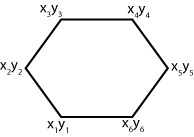
\includegraphics[width = 3 cm]{images/img3.png}
  \end{center}
    
\end{wrapfigure}


Si se conocen objetos obstáculo, se aproximan a polígonos y se almacenan sus vértices. Si uno intersecta el camino de línea recta entre origen y destino, el robot se desplaza a la esquina más cercana y bordea el obstáculo.

\begin{figure}[h!]
	\centering
	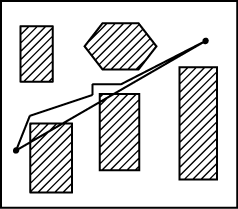
\includegraphics[width=0.35\textwidth]{images/img2.png}
\end{figure}

Se tiene una organización serial, si un modulo falla... 
Se tiene un grupo de sensores para detectar el medio ambiente
\\
\\

\begin{figure}[h!]
	\centering
	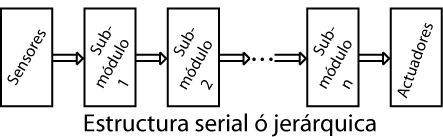
\includegraphics[width=0.55\textwidth]{images/img4.png}
	\label{figura4}
\end{figure}

Este tipo de sistemas no es adecuado para entornos dinámicos y para robots que presentan errores en el movimiento y sensado.



\section{Modelos Reactivos}


Características:

\begin{itemize}
	\item[\textbullet] Basado en el comportamiento de los insectos
	\item[\textbullet] No es necesaria una representación del medio ambiente
	\item[\textbullet] No utiliza planeación de acciones ni de movimiento
	\item[\textbullet] Es adecuado para entornos dinámicos y con errores en el sensado
	\item[\textbullet] Esta basado en comportamientos funcionando en paralelo.
\end{itemize}

\newpage

\begin{figure}[h!]
	\centering
	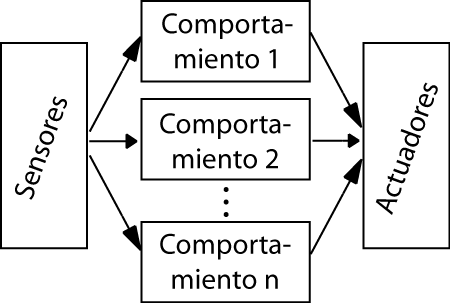
\includegraphics[width=0.5\textwidth]{images/img5.png}
	\label{figura6}
\end{figure}

La salida de cada comportamiento debe ser instantánea a partir del momento que hay una entrada.
Los comportamientos son independientes entre si.
Por ejemplo si se tienen un grupo de robots en un campo con discos con la siguiente programación:

\begin{enumerate}
	\item Moverse aleatoriamente hasta 2 o 3 
	\item Si se encuentra disco y no se porta disco, recoger el disco $\rightarrow1$
	\item Si se encuentra disco y se porta disco soltar el disco $\rightarrow1$
\end{enumerate}



\section{Modelos Híbridos}

Se combinan las arquitecturas tradicionales y reactivas para suplir las deficiencias de cada una de ellos.

\begin{figure}[h!]
	\centering
	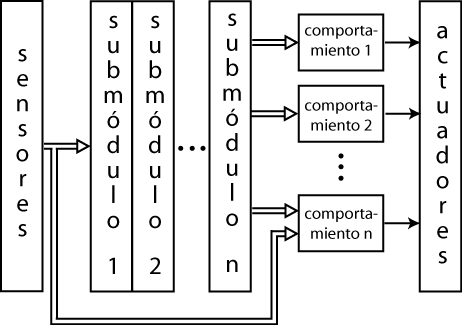
\includegraphics[width=0.5\textwidth]{images/img6.png}
	\label{figura6}
\end{figure}



\section{Comportamientos Reactivos}

Se manejan mediante diagramas estimulo- respuesta o ER

\begin{figure}[h!]
	\centering
	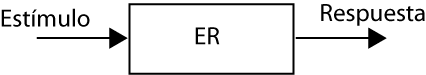
\includegraphics[width=0.4\textwidth]{images/img7.png}
	\label{figura7}
\end{figure}

\paragraph{}
O bien

\begin{figure}[h!]
	\centering
	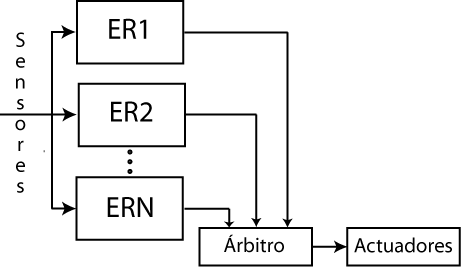
\includegraphics[width=0.5\textwidth]{images/img8.png}
	\label{figura8}
\end{figure}

\paragraph{}
O bien

\begin{figure}[h!]
	\centering
	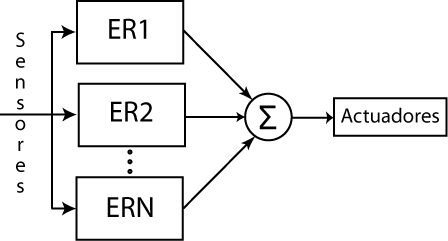
\includegraphics[width=0.5\textwidth]{images/img9.png}
	\label{figura9}
\end{figure}


\paragraph{}

Inteligencia espontánea: los robots hacen algo que no sabrán que estaban haciendo.
En un robot que tiene varios comportamientos coordinados por un agente, todos los comportamientos deben ofrecer una salida por ciclo de reloj, es decir, un comportamiento debe dar salida inmediata.

\begin{figure}[h!]
	\centering
	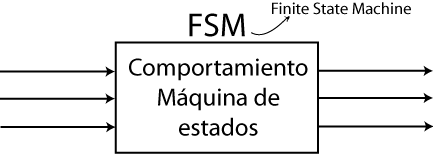
\includegraphics[width=0.5\textwidth]{images/img10.png}
	\label{figura10}
\end{figure}

\paragraph{}
Ronald Brooks propone

\begin{figure}[h!]
	\centering
	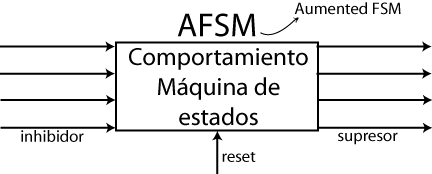
\includegraphics[width=0.5\textwidth]{images/img11.png}
	\label{figura11}
\end{figure}

\paragraph{}
Tenemos entonces:

\begin{figure}[h!]
	\centering
	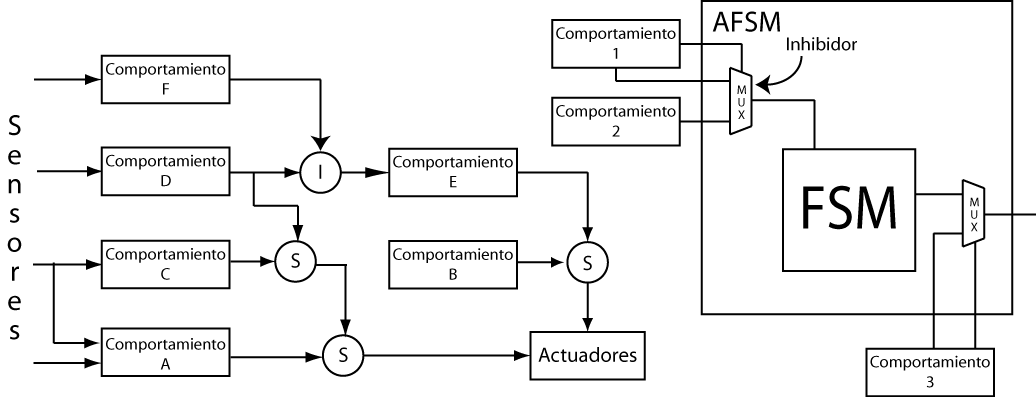
\includegraphics[width=1\textwidth]{images/img12.png}
	\label{figura12}
\end{figure}


\section{Campos Potenciales}

El destino se determina por un capo potencial de atracción y los obstáculos como campos potenciales de repulsión.

\begin{figure}[h!]
	\centering
	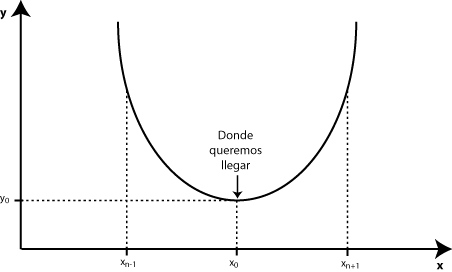
\includegraphics[width=0.5\textwidth]{images/img13.png}
	\label{figura13}
\end{figure}

% NOTA creo que aquí no es x - 1 sino n - 1

$$x_{n} = f(x_{n - 1}) = x_{x - 1} \, \delta \; \dfrac{dy}{dy}$$

Por ejemplo para una parábola \hspace{1cm} $y = y_{0} + (x - x_{0})^2$ 

$$\;\dfrac{dy}{dx} = 2(x - x_{0})$$ 
\hspace{2cm} \textit{si} $\delta = \dfrac{1}{2}$ $\Rightarrow$ $x_{n - 1} = -\dfrac{1}{2} (2(x_{n - 1} - x_{0})) = x_{0}$, \textit{llegamos en un paso}.

\paragraph{}
Esta técnica se conoce como: descendiendo por la pendiente más pronunciada o steppest descent.

\hspace{2cm}$\overline{q}_{n} = [x_n,y_n]$ \hspace{0.5cm} \textit{la posición del robot} \hspace{0.5cm}  $\overline{q}_{n} = \overline{q}_{n - 1} - \delta \overline{f} \left( \overline{q}_{n - 1} \right)$ \hfill \break
\hspace{1cm} \textit{donde} $\overline{f} \left( \overline{q}_{n - 1}\right)$ \textit{es un vector fuerzas unitario en la dirección del gradiente} $\overline{f}(\overline{q}) = \dfrac{\overline{F(\overline{q})}}{\left| \overline{F}(\overline{q})\right|}$ 
\hfill \break
\textit{donde} $\overline{F}(\overline{q}) = \nabla U(\overline{q}) = \left( \dfrac{\partial u}{\partial x} \,\hat{i} + \dfrac{\partial u}{\partial x}\, \hat{j} \right)$ 

El gradiente del campo potencial \hspace{1cm} \textit{donde}  $u(\overline{q}) = U_{\mbox{\textit{atracción}}}(\overline{q}) + U_{\mbox{\textit{repulsión}}}(\overline{q})$

Los campos potenciales atractivos y repulsivos y  $\overline{F}(\overline{q}) = \overline{F}_{atr}(\overline{q}) + \overline{F}_{rep}(\overline{q})$ las fuerzas de atracción y repulsión

\begin{figure}[h!]
	\centering
	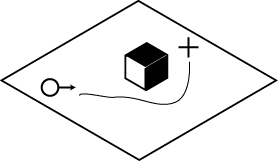
\includegraphics[width=0.5\textwidth]{images/img14.png}
	\label{figura14}
\end{figure}



\section{Campos Potenciales Atractivos}

\begin{center}


$\overline{q} = (x,y)$ \textit{Es la posición del robot}

$\overline{q}_{dest} $ \textit{Posición del punto al que queremos llegar}

$\overline{F}_{atr}(\overline{q}) = \epsilon_{1} (\overline{q} - \overline{q}_{dest})$ \textit{siempre que} $\left| \overline{q} - \overline{q}_{dest} \right| \leq d_{i}$ \textit{para} $\left| \overline{q} - \overline{q}_{dest} \right| > d_{i}$, $U_{atr}(\overline{q}) = \epsilon_{2} \left| \overline{q} - \overline{q}_{dest} \right|$ \textit{o bien,} 
\end{center}

$$U_{atr}(x,y) = \epsilon_{2} \left( (x - x_{0})^2 + (y - y_{0})^2 \right)^\frac{1}{2}$$
$$\dfrac{\partial U_{atr}(x,y)}{\partial x} = \dfrac{\epsilon_{2}2(x - x_{0})}{2\sqrt{(x - x_{d})^2 + (y - y_{d})^2}}$$
$$\dfrac{\partial U_{atr}(x,y)}{\partial y} = \dfrac{\epsilon_{2}(y - y_{0})}{\sqrt{(x - x_{d})^2 + (y - y_{d})^2}}$$
$$\Rightarrow \nabla U_{atr(x,y)} = \dfrac{\epsilon_{2}\left( (x - x_{0}) + (y - y_{d})\right) }{\sqrt{(x - x_{d})^2 + (y - y_{d})^2}} = \dfrac{\epsilon_{2}(\overline{q} - \overline{q}_d)}{\left| \overline{q} - \overline{q}_{d} \right|} = F_{atr}(\overline{q})$$


\section{Campos Potenciales Repulsivos}

\begin{figure}[h!]
	\centering
	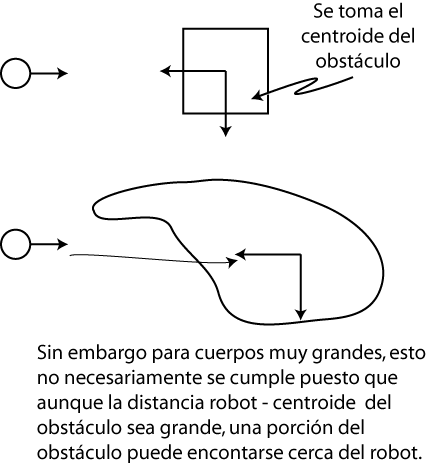
\includegraphics[width=0.7\textwidth]{images/img15.png}
	\label{figura15}
\end{figure}
\newpage

$$\left| \overline{q} - \overline{q}_{obs}\right| \leq d_{0}$$

$$U_{rep}(\overline{q}) = \dfrac{1}{2} \eta \left( \dfrac{1}{\left| \overline{q} - \overline{q}_{obs}\right|}  
- \dfrac{1}{d_{0}} \right)^2$$

$$U_{rep}(x,y) = \dfrac{1}{2} \eta \left( \dfrac{1}{\sqrt{(x - x_{obs})^2 + (y - y_{obs})^2}}  
- \dfrac{1}{d_{0}} \right)^2$$

$$\dfrac{\partial U_{rep}(x,y)}{\partial x} = \eta \left( \dfrac{1}{d_{0}}  
-  \dfrac{1}{\sqrt{(x - x_{obs})^2 + (y - y_{obs})^2}} \right)^2 \left( \dfrac{x - x_{obs}}{\left( (x - x_{obs})^2 + (y - y_{obs})^2 \right)^{\frac{3}{2}}} \right)$$

$$\dfrac{\partial U_{rep}(x,y)}{\partial y} = \eta \left( \dfrac{1}{d_{0}}  
-  \dfrac{1}{\sqrt{(x - x_{obs})^2 + (y - y_{obs})^2}} \right)^2 \left( \dfrac{y - y_{obs}}{\left( (x - x_{obs})^2 + (y - y_{obs})^2 \right)^{\frac{3}{2}}} \right)$$

$$\nabla U_{rep}(\overline{q}) = -\eta \left( \dfrac{1}{\left| \overline{q} - \overline{q}_{obs}\right|} - \dfrac{1}{d_{0}} \right)  \left( \dfrac{1}{\left| \overline{q} - \overline{q}_{obs}\right|^2}\right)  \left( \dfrac{\overline{q} - \overline{q}_{obs}}{\left| \overline{q} - \overline{q}_{obs}\right|}\right) = \overline{F}_{rep}(\overline{q})$$

\paragraph{}
Fuerza de repulsión del obstáculo $k$

\begin{center}
$\overline{F}_{rep}(\overline{q}) = 0$ \textit{ si } $\left| \overline{q} - \overline{q}_{obs}\right| > 0$
\end{center}

$$\overline{F}(\overline{q}) = \overline{F}_{atr}(\overline{q}) + \displaystyle \sum_{i = 1}^{n} \, \overline{F}_{rep}(\overline{q})$$

Luego

$$f(\overline{q}) = \dfrac{\overline{F}(\overline{q})}{\left|  \overline{F}(\overline{q}) \right| }$$


$$\overline{q}_{i + 1} = \overline{q}_{i} - \delta_{i} \overline{f}(q_{i})$$

Ejemplo:

\begin{figure}[h!]
	\centering
	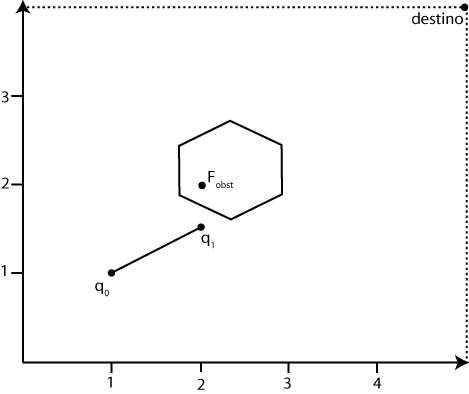
\includegraphics[width=0.7\textwidth]{images/img16.png}
	\label{figura16}
\end{figure}

$$\overline{q}_{0} = (1,1),\, \overline{q}_{obs} = (2,2),\, \overline{q}_{dest} = (5,4),\, d_{0} = 5,\, \epsilon_{1} = 5, \,\, \eta = 2,\, \delta_{0} = 1,\, \delta_{1} = 10$$

$$\overline{F}_{atr}(\overline{q}_{0}) = \overline{F}_{atr}(1,1) = \epsilon_{1}(\overline{q}_{0} - \overline{q}_{dest}) = 1((1,1) - (5,4)) = (-4,-3)$$

$$\overline{F}_{rep}(\overline{q}_{0}) = \left( -2\left( \dfrac{1}{\sqrt{2}} - \dfrac{1}{5} \right) \left( \dfrac{1}{2} \right)  \left( \dfrac{(-1,-1)}{\sqrt{2}} \right) \right) = (0\ldotp3585,0\ldotp3585)$$

$$\overline{F}(\overline{q}) = (-4,-3) + (0\ldotp3585,0\ldotp3585) = (-3\ldotp64,-2\ldotp64)$$

$$f(\overline{q}) = \dfrac{(-3\ldotp64,-2\ldotp64)}{|4\ldotp4985|} = (-0\ldotp8091,-0\ldotp5868)$$
$$ \Rightarrow q_{1} = q_{0} - \delta_{0}\,\overline{f}(\overline{q}_{0}) = (1,1) + (-0\ldotp8091,-0\ldotp5868)$$
$$\Rightarrow q_{1} = (1\ldotp8091,1\ldotp5868)$$

Encontrar los siguientes tres puntos de posicionamiento del robot. Obtenga $q_{2}$, $q_{3}$ y $q_{4}$.


\section{Campos Potenciales Usando Sensores de Proximidad}

\begin{figure}[h!]
	\centering
	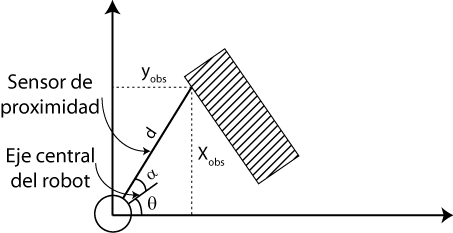
\includegraphics[width=0.7\textwidth]{images/img17.png}
	\label{figura17}
\end{figure}

En el ángulo de determina hacia donde mira el robot respecto a su posición alfa es el ángulo del sensor respecto a la orientación del robot. 

D es la distancia reportada por el sensor al obstáculo. 

$$x_{obs} = d\cos (\theta + \alpha)$$
$$y_{obs} = d\sen (\theta + \alpha)$$
$$\overline{q} - \overline{q}_{obs} = (0,0) - (x_{obs}, y_{obs}) = (-x_{obs}, -y_{obs})$$

\begin{figure}[h!]
	\centering
	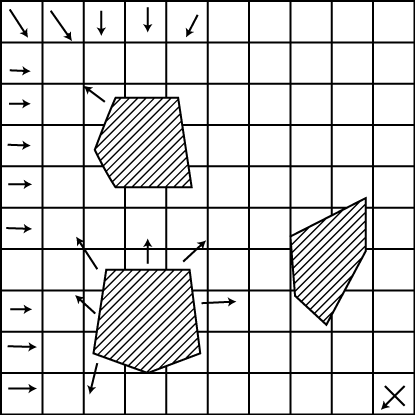
\includegraphics[width=0.5\textwidth]{images/img18.png}
	\label{figura18}
\end{figure}
\newpage

Cuando se conoce la posición de los objetos se puede almacenar en una matriz el campo de repulsión. Esto requiere de un procesador más potente.

\begin{figure}[h!]
	\centering
	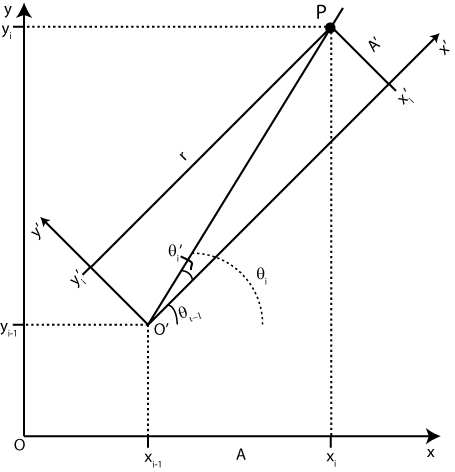
\includegraphics[width=0.5\textwidth]{images/img19.png}
	\label{figura19}
\end{figure}

Dados $(x_{i - 1}, y_{i - 1})$ para llegar al punto $(x_{i}, y_{i})$ se desea saber el ángulo que el robot debe girar para llegar a su destino, o bien el desplazamiento.

$$x_{i} = \overline{OA} = x_{i - 1} + r\cos (\theta_{i - 1} + \theta_{i})$$
$$y_{i} = \overline{AP} = y_{i - 1} + r\sen (\theta_{i - 1} + \theta_{i})$$
$$x_{i} = x_{i}^{\,\prime} \cos (\theta_{i - 1}) - y_{i}^{\,\prime} \sen \theta_{i - 1} + x_{i - 1}$$
$$y_{i} = x_{i}^{\,\prime} \sen (\theta_{i - 1}) - y_{i}^{\,\prime} \cos \theta_{i - 1} + y_{i - 1}$$

Esto para un sistema omnidireccional. En forma matricial:

$$
\begin{bmatrix}
x_{i} \\
y_{i} \\
\theta_{i}
\end{bmatrix} = \begin{bmatrix}
\cos \theta_{i - 1} & \sen \theta_{i - 1} & 0 \\
\sen \theta_{i - 1} & \cos \theta_{i - 1} & 0 \\
0                     &                0      & 1
\end{bmatrix} \begin{bmatrix}
x_{i}^{\,\prime} \\
y_{i}^{\,\prime} \\
\theta_{i}^{\,\prime}
\end{bmatrix} + \begin{bmatrix}
x_{i - 1} \\
y_{i - 1} \\
\theta_{i - 1}
\end{bmatrix}
$$

Despejando, robot omnidireccional

$$
\begin{bmatrix}
x_{i}^{\,\prime} \\
y_{i}^{\, \prime} \\
\theta_{i}^{\, \prime}
\end{bmatrix} = \begin{bmatrix}
\cos \theta_{i - 1} & \sen \theta_{i - 1} & 0 \\
-\sen \theta_{i - 1} & \cos \theta_{i - 1} & 0 \\
0                     &                0      & 1
\end{bmatrix} \begin{bmatrix}
x_{i} - x_{i - 1} \\
y_{i} - y_{i - 1}\\
\theta_{i} - \theta_{i - 1}
\end{bmatrix} 
$$

En el caso de un sistema robot no omnidireccional, las ecuaciones son las mismas, pero la matriz se despeja y queda como sigue:

$$
\begin{bmatrix}
x_{i}^{\,\prime} \\
y_{i}^{\, \prime} \\
\theta_{i}^{\, \prime}
\end{bmatrix} = \begin{bmatrix}
\cos \theta_{i} & \sen \theta_{i} & 0 \\
- \sen \theta_{i} & \cos \theta_{i} & 0 \\
0                     &                0      & 1
\end{bmatrix} \begin{bmatrix}
x_{i} - x_{i - 1} \\
y_{i} - y_{i - 1}\\
\theta_{i} - \theta_{i - 1}
\end{bmatrix} 
$$ 

Ejemplo:

\begin{figure}[h!]
	\centering
	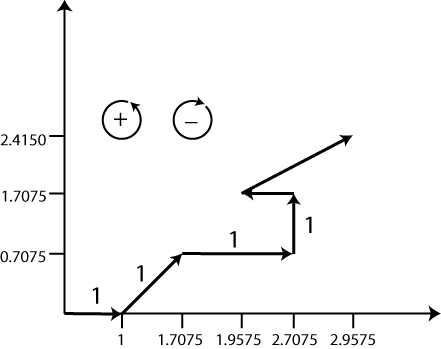
\includegraphics[width=0.5\textwidth]{images/img20.png}
	\label{figura20}
\end{figure}

\textit{tiempo} $i = 1$

$$x_{0} = 0,\, y_{0} = 0, \, \theta_{0} = 0$$
$$x_{1} = 1,\, y_{1} = 0, \, \theta_{1} = 0$$
$$\theta_{i} = \tan^{-1} \left( \dfrac{y_{i} - y_{i - 1}}{x_{i} - x_{i - 1}} \right) $$

Terminar ejercicio.

Caso 1. Robot no omnidireccional

$$x_{1}^{\, \prime} = 1 \cos 0 + 0 \sen 0 = 1$$
$$y_{1}^{\, \prime} = \sen 0 - 0 \cos 0 = 0$$
$$\theta_{1}^{\, \prime} = 0$$
	
$$i = 2$$
$$x_{1} = 1, \, y_{1} = 0, \theta_{1} = 0$$
$$x_{2} = 1\ldotp 7075,\, y_{2} = 0\ldotp 7075, \, \theta_{2} = 45^\circ$$

$$x_{2}^{\, \prime} = 0\ldotp7075 \cos (45^\circ) + 0\ldotp7075 \sen (45^\circ) = 1$$
$$y_{2}^{\, \prime} = 0\ldotp7075 \sen (45^\circ) + 0\ldotp7075 \cos (45^\circ) = 0$$
$$\theta_{2}^{\, \prime} = 45^\circ$$

$$i = 3$$
$$x_{2} = 1\ldotp7075,\, y_{2} = 0\ldotp7075,\, \theta_{2} = 45^\circ$$
$$x_{3} = 2\ldotp7075,\, y_{3} = 0\ldotp7075,\, \theta_{3} = 0$$
$$x_{3}^{\,\prime} = 1 \cos 0 + 0\sen 0 = 1$$
$$y_{3}^{\,\prime} = - 1 \sen 0 + 0\cos 0 = 0$$
$$\theta_{3}^{\,\prime} = -45^\circ$$

Caso 2. Robot omnidireccional 

\textit{tiempo} $i = 1$

$$x_{0} = 0,\, y_{0} = 0,\, \theta_{0} = 0$$
$$x_{1} = 1,\, y_{1} = 0,\, \theta_{1} = 0$$
$$x_{1}^{\,\prime} = 1 \cos 0 + 0\sen 0 = 1$$
$$y_{1}^{\,\prime} = - \sen 0 - 0\cos 0 = 0$$
$$\theta_{1}^{\,\prime} = 0$$

$$i = 2$$
$$x_{1} = 1, \, y_{1} = 0, \theta_{1} = 0$$
$$x_{2} = 1\ldotp7075,\, y_{2} = 0\ldotp7075,\, \theta_{2} = 45^\circ$$
$$x_{2}^{\,\prime} = 0\ldotp7075 \cos 0 + 0\ldotp7075\sen 0 = 0\ldotp7075$$
$$y_{2}^{\,\prime} = - 0\ldotp7075 \sen 0 + 0\ldotp7075\cos 0 = 0\ldotp7075$$
$$\theta_{2}^{\,\prime} = -45^\circ$$

$$i = 3$$
$$x_{2} = 1\ldotp7075, \, y_{2} = 0\ldotp7075, \theta_{2} = 45^\circ$$
$$x_{3} = 2\ldotp7075,\, y_{3} = 0\ldotp7075,\, \theta_{3} = 0$$
$$x_{3}^{\,\prime} = 1 \cos (45^\circ) + 0\sen (45^\circ) = 0\ldotp7075$$
$$y_{3}^{\,\prime} = - 1 \sen (45^\circ) + 0 \cos (45^\circ) = -0\ldotp7075$$
$$\theta_{3}^{\,\prime} = -45^\circ$$



\section{Trayectorias}

$
\begin{array}{cc}
	\mbox{Posición inicial} & \mbox{Velocidades iniciales y finales} \\
	f(0) = 0                & f^{\,\prime}(0) = 0 \\
	f(t_{f}) = x_{i}^{\,\prime} & f^{\,\prime} (t_{f}) = 0 
\end{array}
$

Posición: $f(t) = a_{0} + a_{1}t + a_{2}t^{2} + a_{3}t^{3}$

Mínimo de orden tres para controlar la aceleración.

Velocidad: $f^{\,\prime} (t) = a_{1} + 2a_{2}t + 3a_{3}t^2$

Aceleración: $f^{\,\prime\prime} (t) = 2a_{2} + 6a_{3}t$

$$f(t) = a_{0} + a_{1}t + a_{2}t^{2} + a_{3}t^{3}$$
$$f^{\,\prime} (t) = a_{1} + 2a_{2}t + 3a_{3}t^2$$
$$f^{\,\prime\prime} (t) = 2a_{2} + 6a_{3}t$$

Condiciones lineales para encontrar las constantes:

$$f(0) = 0 = a_{0}$$
$$x_{i}^{\,\prime} = a_{0} + a_{1}t_{f}^{2} + a_{3}t_{f}^{3}$$
$$f^{\,\prime}(0) = a_{1}$$
$$f^{\,\prime}(t_{i}) = 0 = a_{1} + 2a_{2}t_{f} + 3a_{3}t_{f}^{2}$$

$$\Rightarrow a_{2} = \dfrac{3x_{i}}{t_{f}^{2}}$$
$$a_{3} = \dfrac{-2x_{i}}{t_{f}^{3}}$$
	
4 ecuaciones con 4 incógnitas

$$f(t) = a_{0} + a_{1}t + a_{2}t^{2} + a_{3}t^{3} = \dfrac{3x_{i}}{t_{f}^{2}}\,t^{2} - \dfrac{2x_{i}}{t_{f}^{3}}\,t^{3}$$
$$\dot{f}(t) = a_{1} + 2a_{2}t + 3a_{3}t^2 = \dfrac{6x_{i}}{t_{f}^2}\,t - \dfrac{6x_{i}}{t_{f}^3}\, t^2$$
$$\ddot{f} (t) = 2a_{2} + 6a_{3}t = \dfrac{6x_{i}}{t_{f}^2}\,t - \dfrac{12x_{i}}{t_{f}^3}\, t$$

Ejemplo:

$$t_{f} = 3 seg,\, x_{i} = 1$$
$$f(t) = \dfrac{1}{3}\,t^2 - \dfrac{2}{27}\,t^3$$
$$\dot{f}(t) = \dfrac{2}{3}\, t - \dfrac{6}{27}\,t^2$$
$$\ddot{f} = \dfrac{2}{3} - \dfrac{12}{27}\, t$$

%imagen

$$t_{f} = 1seg,\: x_{i}^{\,\prime} = 2,\: y_{i}^{\,\prime} = 5$$


\begin{table}[h!]
	\centering
	\begin{tabular}{c|c|c}
		$t$ & $x^{\,\prime} (t)$ & $y^{\,\prime}(t)$\\\hline
		0 & 0 & 0 \\
		$0\ldotp1$ & $0\ldotp056$ & $0\ldotp14$ \\
		$0\ldotp2$ & $0\ldotp208$ & $0\ldotp52$ \\
		$0\ldotp5$ & 1 & $2\ldotp5$ \\
		$0\ldotp8$ & $1\ldotp792$ & $4\ldotp48$ \\
		1 & 2 & 5
	\end{tabular}
		%\caption{}
\end{table}


$$\left. f(t) = \dfrac{3(2)}{1^2}\, t^2 - \dfrac{2(2)}{1^2}\, t^3\, \right|_{t = 0\ldotp1} = 0\ldotp056 \Leftarrow x$$
$$\left. f(t) = \dfrac{3(5)}{1^2}\, t^2 - \dfrac{2(5)}{1^2}\, t^3\, \right|_{t = 0\ldotp1} = 0\ldotp14 \Leftarrow y$$



\section{Repaso Transformada de Laplace}

$$L\left\lbrace f(t) \right\rbrace = \displaystyle \int_{0}^{\infty} f(t)\,e^{-st}\, dt = F(s)$$

$$\left. L\left\lbrace e^{-\alpha t} \right\rbrace = \displaystyle \int_{0}^{\infty} e^{-\alpha t}\,e^{-st}\, dt = \displaystyle \int_{0}^{\infty} e^{-(s + \alpha)t}\, dt = \dfrac{e^{(s + \alpha)}}{s + \alpha}\right|_{0}^{\infty} = \dfrac{1}{s + \alpha}$$

\textbf{Función escalón}

$$\left. L\left\lbrace u(t) \right\rbrace = \displaystyle \int_{0}^{\infty} e^{-st}\, dt = - \dfrac{e^{st}}{s} \right|_{0}^{\infty} = \dfrac{1}{s}$$

$$ L\left\lbrace \cos (\omega\, t) \right\rbrace = \dfrac{s}{s^2 + \omega^2}$$

$$ L\left\lbrace tu(t) \right\rbrace = L\left\lbrace u_{-1}(t) \right\rbrace = \dfrac{1}{s^2}$$

$$ L\left\lbrace \dfrac{df(t)}{dt} \right\rbrace = sF(s) - \dot{F}(t)$$

$$ L\left\lbrace \displaystyle \int_{0}^{\infty} f(t)\, dt \right\rbrace = \dfrac{1}{s} F(s)$$




\section{Transformada Inversa}

$$f(t) = L^{-1} \left\lbrace F(s) \right\rbrace = \displaystyle \int_{0}^{\infty} F(s)\, e^{st}\, ds$$

Sea la ecuación diferencial

$$\dfrac{d^n\, y(t)}{dt^{n}} + b_{n -1} \dfrac{d^{n - 1}\, y(t)}{dt^{n - 1}} + \ldots + b_{1} \dfrac{dy(t)}{dt} + b_{0}\,y(t)$$

$$= a_{m}\dfrac{d^m\, x(t)}{dt^{m}} + a_{m -1} \dfrac{d^{m - 1}\, x(t)}{dt^{m - 1}} + \ldots + a_{1} \dfrac{dx(t)}{dt} + a_{0}\,x(t)$$

Usando la transformada de \textit{Laplace} para resolver la ecuación diferencial 
(condiciones iniciales nulas).


$$s^{n}Y(s) + b_{n - 1}s^{n - 1}Y(s) + \ldots + b_{1}sY(s) + b_{0}Y(s) = $$
$$a_{m}s^{m}X(s) + a_{m - 1}s^{m - 1}X(s) + \ldots + a_{1}sX(s) + a_{0}X(s)$$

$$\Rightarrow (s^n + b_{n - 1} s^{n -1} + \ldots + b_{1}s + b_{0}) Y(s) = (a_{m}s^m + a_{m - 1}s^{m - 1} + \ldots + a_{1}s + a_{0})X(s)$$

$$\Rightarrow \dfrac{Y(s)}{X(s)} = \dfrac{a_{m}s^m + a_{m - 1}s^{m - 1} + \ldots + a_{1}s + a_{0}}{s^n + b_{n - 1} s^{n -1} + \ldots + b_{1}s + b_{0}}$$

Se resuelve por fracciones parciales

\section{Fracciones Parciales}

$$F(s) = \dfrac{P(s)}{Q(s)} = \dfrac{P(s)}{s(s - s_{1})(s - s_{2})\cdots (s - s_{n})}$$
$$= \dfrac{A_{_0}}{s} + \dfrac{A_{_1}}{s - s_{_1}} + \dfrac{A_{_2}}{s - s_{_2}} + \ldots 
+ \dfrac{A_{n}}{s - s_{n}}$$

$$\Rightarrow f(t) = A_{_0} + A_{_1}e^{s_{_1} t} + A_{_2}e^{s_{_2} t} + \ldots + A_{n}e^{s_{n} t}$$

$$(s - s_{k})F(s) = \dfrac{(s  s_{k})P(s)}{Q(s)}$$

$$= \dfrac{(s - s_{k})}{s}A_{_0} +\dfrac{(s - s_{k})}{s - s_{_1}}A_{_1} + \ldots + \dfrac{(s - S_{k})}{s - s_{k}}A_{k} + \ldots + 
			\dfrac{(s - s_{k})}{s - s_{n}}A_{n}$$

$$= \dfrac{(s - s_{k})}{s}A_{_0} +\dfrac{(s - s_{k})}{s - s_{_1}}A_{_1} + \ldots + A_{k} + \ldots + 
\dfrac{(s - s_{k})}{s - s_{n}}A_{n}$$

Si $s = s_{k}$

$$ A_{k} = \left[ (s - s_{k}) \dfrac{P(s)}{Q(S)} \right]_{s = s_{_k}} $$

\textbf{Ejemplo}

$$F(s) = \dfrac{s + 2}{s(s + 1)(s + 2)}$$

$$A_{_0} = \left[ \dfrac{s(s + 2)}{s(s + 1)(s + 3)} \right]_{s = 0} = \dfrac{2}{3} $$

$$A_{_1} = \left[ \dfrac{(s + 1)(s + 2)}{s(s + 1)(s + 3)} \right]_{s = -1} = - \dfrac{1}{2} $$

$$A_{_2} = \left[ \dfrac{(s + 3)(s + 2)}{s(s + 1)(s + 3)} \right]_{s = -3} = - \dfrac{1}{6} $$

$$F(s) = \dfrac{\frac{2}{3}}{s} - \dfrac{\frac{1}{2}}{s + 1} - \dfrac{\frac{1}{6}}{s + 3}$$

$$\Rightarrow f(t) = \dfrac{2}{3} - \dfrac{1}{3} e^{-t} - \dfrac{1}{6} e^{-3t}$$

%imagen




\section{Polos Rales Múltiples}

$$F(s) = \dfrac{P(s)}{(s - s_{_1})^2 (s - s_{_2})}$$

$$= \dfrac{A_{_{13}}}{(s - s_{_1})^3} + \dfrac{A_{_{12}}}{(s - s_{_1})^2} + \dfrac{A_{_{11}}}{s - s_{_1}} + \dfrac{A_{_2}}{s - s_{_2}}$$

Transformada inversa

$$f(t) = A_{_{13}} \dfrac{t^2}{2} e^{s_{_1} t} + A_{_{12}}\, t \, e^{s_{_1} t} + A_{_{11}}\,e^{s_{_1} t} + A_{_2}\, e^{s_{_2} t}$$

Ejemplo

$$F(s) = \dfrac{1}{(s + 2)^3 (s + 3)} = \dfrac{A_{_{13}}}{(s + 2)^3} + \dfrac{A_{_{12}}}{(s + 2)^2} + \dfrac{A_{_{11}}}{s + 2} + \dfrac{A_{_2}}{s + 3}$$

$$A_{_{13}} \left[ (s + 3)^3 F(S) \right]_{s = -2} = \left[ A_{_{13}} + A_{_{12}}(s + 2)^2 + \dfrac{A_{_2} (s + 2)^3}{s + 3} \right]_{s = -2}$$

Valuando con $A_{_{13}} = 1$

$$A_{_{12}} = \left[ (s + 2)^2 F(S) \right]_{s = -2} = \left[ \dfrac{A_{_{13}}}{s + 2} + A_{_{12}} + A_{_{11}}(s + 2) =\dfrac{A_{_2}(s + 2)^2}{s + 3} \right]_{s = -2}$$

Existe una indeterminación en el primer término. Sin embargo, se puede demostrar que

$$A_{_{12}} = \left[ \dfrac{d}{ds}\left( (s + 2)^3\, F(s) \right) \right]_{s = -2}  = \dfrac{d}{ds}\left( \dfrac{1}{s + 3} \right) $$

$$= \left. \dfrac{d}{ds} \left( A_{_{13}} + A_{_{12}}(s + 2) + A_{_{11}}(s + 2)^2 + \dfrac{A_{_{2}}(s + 2)^3 }{s + 3}\right)  \right|_{s = -2} $$

$$\Rightarrow \dfrac{d}{ds} \left( \dfrac{1}{s + 3} \right) = A_{_{12}}$$

$$\Rightarrow A_{_{12}} = \left. \dfrac{-1}{(s + 3)^2} \right]_{s = -2} = - 1$$

Luego, para $A_{_{11}}$

$$A_{_{11}} \dfrac{1}{2}\,\dfrac{d^2}{ds^2} \left[ (s + 2)^2\,F(s) \right]_{s = -2} = \left.  \dfrac{1}{2}\, \dfrac{2}{(s + 3)^3} \right|_{s = -2} = 1$$

$$\therefore\:\: A_{q}(r - k) = \left\lbrace \dfrac{1}{k!}\,\dfrac{d^k}{ds^k} \left[ (s - s_{q})^r \, \dfrac{P(s)}{Q(s)} \right] \right\rbrace_{s = s_{q}}$$

$$\Rightarrow F(s) = \dfrac{1}{(s + 2)^3} - \dfrac{1}{(s + 2)^2} + \dfrac{1}{s + 2} - \dfrac{1}{s + 3}$$

$$\therefore \:\: f(t) = \dfrac{1}{2}\, t^2 e^{-2t} - te^{-2t} + e^{-2t} - e^{-3t}$$


\section{Polos Complejos Conjugados}

$$F(s) = \dfrac{P(s)}{(s^2 + 2\zeta \omega_{n}s + \omega_{n}^2)(s - s_{_{3}})}$$

$$= \dfrac{A_{_{1}}}{s + \zeta \omega_{n} - j\omega_{n} \sqrt{1 - \zeta^2}} + \dfrac{A_{_{2}}}{s + \zeta \omega_{n} - j\omega_{n} \sqrt{1 - \zeta^2}} + \dfrac{A_{_{3}}}{s + s_{_3}}$$

Como $As^2 + Bs + C = s^2 + 2\zeta \omega_{n}s +\omega_{n}^{2}$, $\: s_{1,2} = \dfrac{- b \pm \sqrt{b^2 - 4ac}}{2a}.$

La transformada inversa de $F(s)$ es

$$f(t) = A_{_{1}} e^{- \left( \zeta \omega_{n} + j\omega_{n} \sqrt{1 - \zeta^2} \right)t } + A_{_2} e^{- \left( \zeta \omega_{n} - j\omega_{n} \sqrt{1 - \zeta^2} \right)t } + A_{_3} e^{s_{_3} t}$$

Eliminando los coeficientes complejos

$$f(t) = 2 |A_{_1}| e^{-\zeta \omega_{n}t} \sen \left( \omega_{n} \sqrt{1 - \zeta^2 t} + \phi \right) + A_{_3}e^{s_{_3}t}$$

$$\phi = \mbox{Ángulo de } A_{_1} + 90^\circ$$

$$A_{_1} = \left[ (s - s_1)F(s)\right]_{s = s_{_1}} = a_{_{1Re}} + a_{_{1Im}}$$

$$|A_{_1}| = \sqrt{a_{_{1Re}}^2 + a_{_{1Im}}^2}$$

$$deg(A_{_1}) = \tan^{-1} \left( \dfrac{a_{_{1Re}}}{a_{_{1Im}}} \right) $$

Ejemplo

$$F(s) = \dfrac{10}{(s^2 + 6s + 25)(s + 2)} = \dfrac{A_{_1}}{s + 3 - j4} + \dfrac{A_{_2}}{s + 3 + j4} + \dfrac{A_{_3}}{s + 2}$$

$$A_{_1} = \left[ (s + 3 - j4) F(s) \right]_{s = 3 + j4} = \left. \dfrac{10}{(s + 3 + j4)(s + 2)} \right|_{s = 3 + j4}$$

$$= \dfrac{10}{(j8)(-1 + j4)} = \dfrac{10}{-32 - j8}$$

Multiplicando por el conjugado

$$\dfrac{10(-32 + j8)}{(-32 - j8)(-32 + j8)} = \dfrac{-10}{8(17)}(4 - j)$$

$$|A_{_1}| = \dfrac{10}{8(17)} \sqrt{16 + 1} = 0\ldotp303$$

$$deg(A_{_1}) = 194^\circ \Rightarrow \phi = -104^\circ$$

$$A_{_3} = \left[ (s + 2)F(s) \right]_{s = -2} = 0\ldotp59$$

$$\Rightarrow f(t) = 0\ldotp6 e^{-3t} \sen (4t - 104^\circ) + 0\ldotp59 e^{-2t}$$

%imagen


\section{Motores de Corriente Directa}

%imagen

$$v(t) = Ri(t) + L \dfrac{di(t)}{dt} + \epsilon(t)$$

$$\epsilon(t) = \mbox{Voltaje de fuerza electromotriz } = k_{m}\omega(t)$$ 

Por \textit{Laplace}
$$V(s) = (R + Ls)I(s) + \epsilon(s)$$

Pero

$$\tau_{a}(s) = k_{m}I(s)$$

$$\tau_{l}(s) = Js\omega(s) + f\omega (s)$$

$$\tau_{l} \sqcup \mbox{ Torque de aplicación}$$
$$J \sqcap \mbox{ Momento de incercia}$$
$$f \sqsubset \mbox{ Coeficiente de fricción}$$

%imagen

$$\omega(s) = \dfrac{\tau_{a}}{Js + f}$$

$$\Rightarrow \omega(s) = \dfrac{k_{m}I(s)}{Js + f} = \dfrac{k_{m} \dfrac{V(s) - \epsilon (s)}{R + Ls}}{Js + f}$$

$$\omega(s) = \dfrac{k_{m} V(s) - k_{m}^{2}\omega(s)}{(Js + f)(R + Ls)}$$

$$\Rightarrow \omega(s) = \dfrac{k_{m}V(s)}{(Js + f)(R + Ls) + k_{m}^{2}}$$

$$\Rightarrow \dfrac{\omega(s)}{V(s)} = \dfrac{k_{m}}{(Js + f)(R + Ls) + k_{m}^{2}} = \dfrac{s\theta(s)}{V(s)}$$

$$\Rightarrow \dfrac{\theta(s)}{V(s)} = \dfrac{k_{m}}{s(k_{m}^{2} + (Js + f)(R + Ls))}$$

Se puede hacer la siguiente simplificación

$$\dfrac{\theta(s)}{V(s)} = \dfrac{k_{_{0}}}{s(s + \alpha)}$$

%imagen

$$F(V(t)) = \displaystyle \int_{0}^{t_{_{1}}}\, V_{p}\,e^{-st}\, dt = \left. - \dfrac{V_{p}\,e^{-st}}{s} \right|_{0}^{t_{_{1}}} = V_{p} \left( \dfrac{1 - e^{-st_{_{1}}}}{s} \right) $$

$$\theta(s) = V(s)H(s) = \left( \dfrac{k_{_{0}}}{s(s + \alpha)} \right) \left( \dfrac{V_{p}(1 - e^{-st_{_{1}}})}{s} \right)  $$

$$\theta(s) = \dfrac{k_{_{0}}V_{p}(1 - e^{-st_{1}})}{s^2(s + \alpha)}$$

Por fracciones parciales

$$\Rightarrow \dfrac{A_{_{12}}}{s^2} + \dfrac{A_{_{11}}}{s} + \dfrac{A_{_{2}}}{s + \alpha}$$

$$\theta(t) = A_{_{12}} te^{-t} + A_{11}e^{-t} + A_{_{2}}e^{-\alpha t}$$

Encontrar $A_{_{11}}$, $A_{_{12}}$ y $A_{_{2}}$

%imagen

Implementar $A_{_12}te^{-t} + A_{_{11}}e^{-t} + A_{_{2}}e^{-\alpha t}$ requiere de amplificadores operacionales y condensadores, en configuración integrador y/o derivador; luego entonces es cero y cinviene hacerlo digital.


\section{Transformada Z}

$$Z\left[ x[n] \right] = \displaystyle \sum_{n = -\infty}^{\infty}\, x[n]z^{-n} = X(z)$$

%imagen

Representar $3\ldotp76$ a 8 bits, 4 enteros y 4 decimales

\begin{table}
	\begin{tabular}{ccccccccc}
		$2^3$ & $2^2$ & $2$ & $2^0$ & $\cdotp$ & $2^{-1}$ & $2^{-2}$ & $2^{-3}$ & $2^{-4}$    \\
		$0$ & $0$ & $1$ & $1$ & $\cdotp$ & $1$ & $1$ & $0$ & $0$
	\end{tabular}
\end{table}

$Z$ es un número complejo limitado a un número de convergencia.

$$\Rightarrow Z\left\lbrace x[n - 1] \right\rbrace = \displaystyle \sum_{-\infty}^{\infty}\, x[n - 1]z^{-n}$$

$$k = n - 1$$
$$n = -\infty \:\:\: k = -\infty$$
$$n = \infty \:\:\: k = \infty$$
$$n = k + 1$$

$$Z\left\lbrace x[n - 1] \right\rbrace = \displaystyle \sum_{- \infty}^{\infty} \, x[k]z^{-(k + 1)} = z^{-1} \displaystyle \sum_{-\infty}^{\infty} x[k]z^{-k} = z^{-1} X(z)$$

De manera similar

$$Z\left\lbrace x[n - 1] \right\rbrace = zX(z)$$


\section{Ecuación en Diferencias}

$$a_{n}y[n - N] + a_{n - 1}y[n - (N - 1)] + \ldots + a_{_0}y[n] = $$
$$b_{m}x[n - N] + b_{m - 1}x[n - (N - 1)] + \ldots + b_{_0}x[n]$$
 
Análogo a la ecuación

$$c_{n} \dfrac{d^{n} y(t)}{dt^{n}} + \ldots + c_{_0}y(t) = $$
$$d_{m} \dfrac{d^{m} x(t)}{dt^{m}} + \ldots + d_{_0}y(t)$$

%imagen

Se requiere una función que transforme de \textit{Laplace} a $Z$ ($s \rightarrow z$) conservando los polos estables.

Esta función es la función Bilineal,

$$s = \dfrac{2}{T} \left( \dfrac{z - 1}{z + 1} \right)$$

$$H(z) = \left. H(s) \right|_{s = \dfrac{2}{T} \left( \dfrac{z - 1}{z + 1} \right)}$$

$$\mbox{Si } H(s) = \dfrac{k_{_0}}{s(s + \alpha)}$$

$$\Rightarrow H(z) = \left. \dfrac{k_{_0}}{s(s + \alpha)} \right|_{s = \dfrac{2}{T} \left( \dfrac{z - 1}{z + 1} \right)}$$

$$H(z) = \dfrac{k_{_0}}{\left( \dfrac{2(z - 1)}{T(z + 1)} \right) \left( \dfrac{2(z - 1)}{T(z + 1)}  + \alpha \right)}$$

$$H(z) = \dfrac{k_{_0}}{\dfrac{4(z - 1)^{2}}{T^{2}(z + 1)^{2}} + \dfrac{2(z - 1)}{T(z + 1)} + \alpha}$$

$$= \dfrac{k_{_0}T^{2}(z^{2} + 2z + 1)}{z^{2}(2T\alpha + 4) - 8z + 4 -2T\alpha}$$

Multiplicando por $\dfrac{z^{-2}}{z^{-2}}$

$$= \dfrac{k_{_0}T^{2}(1 + 2z^{-1} + z^{-2})}{(2T\alpha + 4) - 8z^{-1} + (4 - 2T\alpha)z^{-2}} = \dfrac{\theta (z)}{V(z)}$$

$$V(z)\left[ k_{_0}T^{2}(1 + 2z^{-1} + z^{-2}) \right] = \theta(z) \left[ (2T\alpha + 4) - 8z^{-1} + (4 - 2T\alpha)z^{-2} \right]$$

$$Z^{-1} \left\lbrace  V(z) \right\rbrace = v(n)$$

Antitransformando

$$K_{_0}T^{2}v[n] + 2k_{_0}T^{2}v[n - 1] + k_{_0}T^{2}v[n -2] = \theta[n] (2T\alpha + 4) - 8\theta[n - 1] + (4 - 2T\alpha)\theta[n - 2]$$



\section{Repaso Matemática Discreta}


El impulso

%imagen

%imagen

$$x_{k} = \ldots + x_{_{-2}}\delta_{k + 2} + x_{_{-1}}\delta_{k + 1} + x_{_0} \delta_{k} + x_{_1}\delta_{k - 1} + x_{_2}\delta_{k - 2} \Rightarrow x_{k} = \sum_{i = -\infty}^{\infty}\, x_{i}\delta_{k - i}$$

$x_{k} \rightarrow $ Función.

$x_{i} \rightarrow $ Constante.

En el mundo continuo

%imagen

Pero en el discreto:

%imagen

Se espera que 

%imagen

En general una espuesta lineal

%imagen

Como 

$$T\left\lbrace \delta_{k - 1} \right\rbrace = h_{k}$$

%imagen

En el continuo:

$$a_{n}\dfrac{d^{n}y(t)}{dt^{n}} + a_{n - 1}\dfrac{d^{n - 1}y(t)}{dt^{n - 1}} + \ldots + a_{_0}y(t) = $$

$$b_{_0}x(t) + b_{_1}\dfrac{dx(t)}{dt} + \ldots + b_{m} \dfrac{d^{m}x(t)}{dt^{m}}$$

$$\Rightarrow Y(s)(a_{n}s^{n} + a_{n - 1}s^{n - 1} + \ldots + a_{_0}) = $$
$$X(s)(b_{_0} + b_{_1}s + \ldots + b_{m}s^{m})$$

$$\Rightarrow Y(s) = \dfrac{X(s)(b_{_0} + b_{_1}s + \ldots + b_{m}s^{m})}{a_{n}s^{n} + a_{n - 1}s^{n - 1} + \ldots + a_{_0}}$$

$$= \dfrac{A_{_0}}{s + s_{_0}} + \dfrac{A_{_1}}{s + s_{_1}} + \ldots + \dfrac{A_{n}}{s + s_{n}}$$

$y(t) = \ldots$

En el discreto:

$$x_{k} = 2^k U_{k}$$

\[
U_{k} = \left\{
\begin{array}{lcl}
1 & \mbox{	si } & k\geq 0 \\
  &              &         \\    
0 & \mbox{ si }  & k < 0
\end{array}
\right.
\]

$$x(z) = \sum_{k = -\infty}^{\infty}\, x_{k}z^{-k} = \sum_{k = 0}^{\infty}\, 2^{k}z^{-k} = \sum_{k = 0}^{\infty}\, (2^{-1}z)^{-k}$$

Multimplicando ambos lados por $(2^{-1}z)^{-1}$

$$(2^{-1}z)^{-1} X(z) = \sum_{k = 0}^{\infty}\, (2^{-1}z)^{-1}(2^{-1}z)^{-k} = \sum_{k = 0}^{\infty}\, (2^{-1}z)^{-(k + 1)}$$

si $i = k + 1\, \Rightarrow \, k = 0;\, i = 1,\, k = \infty;\, i = \infty.$ 

$$(2^{-1}z)^{-1} X(z) = \sum_{k = 1}^{\infty}\, (2^{-1}z)^{-i}$$

Como $i$ es variable muda, se puede

$$(2^{-1}z)^{-1} X(z) = \sum_{k = 1}^{\infty}\, (2^{-1}z)^{-k}$$

Restando a la ecuación original

$$X(z) - (2^{-1}z)^{-1}X(z) = \sum_{k = 0}^{\infty}\, (2^{-1}z)^{-k} - \sum_{k = 1}^{\infty}\, (2^{-1}z)^{-k}$$

$$X(z) - (2^{-1}z)^{-1}X(z)  =  1$$

Despejando

$$X(z) = \dfrac{1}{1 - 2z^{-1}} \leftrightarrow 2^{k}$$

Volviendo con el robot

$$\dfrac{\theta(s)}{V(s)} = \dfrac{k_{_0}}{s(s + \alpha)} = H(s)$$

$$s = \dfrac{2}{T}\left( \dfrac{z - 1}{z + 1} \right)$$ 

$$H(z) = \left. H(s)\right|_{s = \dfrac{2}{T}\left( \dfrac{z - 1}{z + 1} \right)}$$

$$\dfrac{\theta(s)}{V(z)} = \dfrac{k_{_0}T^{2}(1 + 2z^{-1} + z^{-2})}{(sT\alpha + 4) - 8z^{-1} + (4 - 2T\alpha)z^{-2}}$$
	
$$\theta(z)\left( (2T\alpha + 4) - 8z^{-1} + (4 - 2T\alpha)z^{-2} \right) = V(z)\left( k_{_0}T^{2}(1 + 2z^{-1} + z^{-2}) \right)$$	

Antitransformando

$$(2T\alpha + 4)\theta_{n} - 8\theta_{n - 1} + (4 - 2T\alpha)\theta_{n - 2} = k_{_0}T^{2}(V_{n} + 2V_{n - 1} + V_{n - 2})$$ 

Despejando $\theta_{n}$

$$\theta_{n} = \dfrac{k_{_0}T^{2}(V_{n} + V_{n - 1} + V_{n - 2}) + 8\theta_{n - 1} - \theta_{n - 2}(4 - sT\alpha)}{2T\alpha + 4}$$


\section{Movimiento en las llantas}

%imagen

$J_{w} = $ Momento de inercia de la llanta.

$\ddot{\theta}_{w} = $ Aceleración rotacional de la llanta.

$m_{w} = $ Masa de la llanta.

$F_{R} = $ Fuerza de fricción $= B_{w} \dot{\theta}_{w}$.

$B_{w} = $ Constante de fricción.

$R_{w} = $ Radio de la llanta.



\textbf{Torque de la llanta}:


$\tau_{w} = J_{w}\ddot{\theta}_{w} + B_{w}\dot{\theta}_{w}$

$\tau_{w} = F_{w}R_{w}$

$F_{w} = \dfrac{\tau_{w}}{R_{w}} = \dfrac{1}{R_{w}}\left( J_{w}\ddot{\theta}_{w} + B_{w}\dot{\theta}_{w} \right)$ 




\section{Movimiento Lineal de Robot}

$\ddot{x}_{R} = $ Aceleración lineal del robot.

$m_{R} = $ Masa del robot.

$F = m_{R}\ddot{x}_{R}$.

Se tiene dos llantas

$F = F_{wI} + F_{wD} = m_{R}\ddot{x}_{R} = m_{R}\dot{v}_{R}$

$\Rightarrow$

$\dfrac{1}{R_{wI}} \left( J_{wI}\ddot{\theta}_{wI} + B_{wI}\dot{\theta}_{wI}\right) + \dfrac{1}{R_{wD}} \left( J_{wD}\ddot{\theta}_{wD} + B_{wD}\dot{\theta}_{wD}\right)???????$

$\Rightarrow$


$$V_{R}(s) = \omega_{wI}(s)\left( \dfrac{J_{wI}s + b_{wI}}{m_{R}R_{wI}s} \right) + \omega_{wD}(s)\left( \dfrac{J_{wD}s + b_{wD}}{m_{R}R_{wD}s} \right)$$

$
V(s) = \begin{bmatrix}
\dfrac{J_{wI}s + b_{wI}}{m_{R}R_{wI}s} & \dfrac{J_{wD}s + b_{wD}}{m_{R}R_{wD}s}  
\end{bmatrix} \begin{bmatrix}
 \omega_{wI}(s) \\
 \omega_{wD}(s)  
\end{bmatrix}
$


\section{Movimiento Rotacional del Robot}

$J_{R} = $ Momento de inercia del robot.

$R_{R} = $ Radio del robot.

$\ddot{\theta}_{R} = $ Aceleración rotacional del robot.

$\tau_{R} = $ Torque del robot.

$B_{R} = $ Constante de fricción.

$\tau_{R} = J_{R}\ddot{\theta}_{R} + B_{R}\dot{\theta}_{R} = (F_{wI} - F_{wD}) R_{R} = \left( \dfrac{J_{R}\ddot{\theta}_{R} + B_{R}\dot{\theta}_{R}}{R_{wI}} \right) R_{R} - \left( \dfrac{J_{R}\ddot{\theta}_{R} + B_{R}\dot{\theta}_{R}}{R_{wD}} \right)R_{R}$

Transformando

$\tau_{R}(s) = \omega_{R}(s)(sJ_{R} + R_{R})$

$\omega_{R}(s) = \dfrac{\omega_{wI}(s)R_{R}}{R_{wI}} \left( \dfrac{J_{wI}s + \omega_{wI}}{J_{R}s + B_{R}} \right) - \dfrac{\omega_{wD}(s)R_{R}}{R_{wD}} \left( \dfrac{J_{wD}s + \omega_{wD}}{J_{R}s + B_{R}} \right)$

\[
\omega_{R}(s) = 
\begin{bmatrix}
\dfrac{R_{R}}{R_{wI}}  \left( \dfrac{J_{wI}s + \omega_{wI}}{J_{R}s + B_{R}} \right) \\
-\dfrac{R_{R}}{R_{wD}} \left( \dfrac{J_{wD}s + \omega_{wD}}{J_{R}s + B_{R}} \right) 
\end{bmatrix}^{T} \begin{bmatrix}
\omega_{wI}(s) \\
\omega_{wD}(s)
\end{bmatrix}
\]


\section{Movimiento del Robot}

Juntando el moviento lineal con el rotacional


\[
\begin{bmatrix}
V_{R}(s) \\
\omega_{R}(s)
\end{bmatrix} = \begin{bmatrix}
\dfrac{J_{wI}s + b_{wI}}{m_{R}R_{wI}s} & \dfrac{R_{R}}{R_{wI}} \left( \dfrac{J_{wI}s + \omega_{wI}}{J_{R}s + B_{R}} \right) \\
                                       &    \\
\dfrac{J_{wD}s + b_{wD}}{m_{R}R_{wD}s} & -\dfrac{R_{R}}{R_{wD}} \left( \dfrac{J_{wD}s + \omega_{wD}}{J_{R}s + B_{R}} \right)
\end{bmatrix}^{T} \begin{bmatrix}
\omega_{wI}(s) \\
\omega_{wD}(s)
\end{bmatrix}
\]

Por medio de la matriz inversa se despeja 
$
\begin{bmatrix}
\omega_{wI}(s) \\
\omega_{wD}(s)
\end{bmatrix}
$

\[
\begin{bmatrix}
\omega_{wI}(s) \\
\omega_{wD}(s)
\end{bmatrix} = A^{-1} \begin{bmatrix}
V_{R}(s) \\
\omega_{R}(s)
\end{bmatrix}
\]

El modelo de motor despreciando la fricción

\[
\begin{bmatrix}
\omega_{wI}(s) \\
\omega_{wD}(s)
\end{bmatrix} = \begin{bmatrix} \dfrac{k_{01}V_{1}(s)}{s+\alpha_{1}}\\ \dfrac{k_{0D}V_{D}(s)}{s+\alpha_{D}}
\end{bmatrix}
\]

Voltaje que se tiene que aplica a los motores

\[
\begin{bmatrix}
V_{1}(s) \\
V_{D}(s)
\end{bmatrix} = \begin{bmatrix} \dfrac{\omega_{1}(s)(s+\alpha_{1})}{k_{01}}\\ \dfrac{\omega_{D}(s)(s+\alpha_{D})}{k_{0D}}
\end{bmatrix}
\]

\section{Cinemática del Robot}

%imagen
Número de tics del encoder para una vuelta complera de la llanta.

%imagen

%imagen

$$S_{L} = 2 \pi r\frac{ticks{L}}{ticks_per_rev}$$

Análogo para $S_{R}$

$$S=\frac{(S_{L}+S_{R})}{2}$$

%imagen

$$S_{L}=\phi(c+\frac{d}{2})$$
$$S_{R}=\phi(c-\frac{d}{2})$$

$$S_{L} - S_{D} \, = \phi\,d \hspace{0.5cm}  \Rightarrow \hspace{0.5cm} \phi \,= \frac{S_{L} - S_{R}}{d}$$
	
	
$$V_{R}=2\pi r \dot{\theta_{R}} = 2 \pi r \omega_{R} $$

$$V_{L}=2\pi r \dot{\theta_{L}} = 2 \pi r \omega_{L} $$

Velocidad angular

$$\omega = \frac{2\pi r}{d}(\omega_{L}-\omega_{D})$$

$$v=v_{R} + v_{L}$$

$$
\begin{bmatrix}
V \\
\omega
\end{bmatrix} = 2 \pi r \begin{bmatrix} \dfrac{1}{2} & \dfrac{1}{2} \\ \\ \dfrac{-1}{d} & \dfrac{d}{2} 
\end{bmatrix} \begin{bmatrix} V \\ \omega
\end{bmatrix}
$$

$$
\begin{bmatrix}
\omega_{R} \\
\omega_{L}
\end{bmatrix} = \dfrac{1}{2\pi r} \begin{bmatrix} 1 & \dfrac{-d}{2} \\
 \\ 1 & \dfrac{d}{2} 
\end{bmatrix} \begin{bmatrix} V \\ \omega
\end{bmatrix}
$$



\section{Control ON - Off}
El motor se prende o se apaga dependiendo de si la velocidad del motor esta abajo o arriba de la velocidad deseada.

$R(t) = $ Función que controla el motor

$V_{act}(t) = $ Velocidad del moto

$V_{des}(t) = $ Velocidad deseada

$k_{c} = $ Valor de la constante del control

$$
R(t) = \begin{cases}
k_{c}  \hspace{0.3cm}  & si \hspace{0.3cm}  V_{act}(t) < V_{des}(t) \\
0 & si  \hspace{0.3cm}  V_{act}(t) \geq V_{des}(t)
\end{cases}
$$

%imagen

\section{Control Proporcional}

$$
R(t) = k_{p} (v_{des}(t)-v_{act}(t))
$$
%imagen 

\section{Control Integral Proporcional}

La idea del controlador I es reducir el error del estado estable del controlador P. 
$$
R(t) = k_{p} [  \,e(t)+ \dfrac{1}{T_{1}}\int_{0}^{t} \! e(t) \,dt\, ]
$$

Discretizando: regla trapezoidal

$$
R_{n} = k_{p} e_{n} + \dfrac{k_{p}}{T_{1}} \, t_{\Delta} \, \sum_{i=1}^{n} \dfrac{e_{i}-e_{i-1}}{2}
$$

Si se calcula \hspace{0.3cm}  

$R_{n}-R_{n-1}$

$$R_{n}-R_{n-1} =\, k_{p}(e_{n}-e_{n-1}) + \dfrac{k_{p}}{T_{I}} \, t_{\Delta}(\dfrac{e_{n}-e_{n-1}}{2})
$$
	
$$
k_{I} = \dfrac{k_p}{t_I} t_{\Delta} \hspace{0.5cm} \Rightarrow \hspace{0.5cm} R_n= \, R_{n-1} + k_p(e_n - e_{n-1}) + k_1 \, (\dfrac{e_n - e_{n-1}}{2}
$$

Reduce el error en estado estable.

\section{Control Derivativo Proporcional}

$$
R(t)= k_p \left [(t)+ T_D \dfrac{d}{dt} e(t) \right ]
$$

CONTROL PID

$$
R(t)=k_p \left [e(t)+ \dfrac{1}{T_1} \int_{0}^{1} e(t) \, dt + T_D \dfrac{d}{dt} \, e(t) \right ]
$$

En el discreto

$$
R_{n} = k_{p} e_{n} + \dfrac{k_{p}}{T_{I}} \,\, t_{\Delta} \, \sum_{i=1}^{n} \dfrac{e_{i}-e_{i-1}}{2} + \dfrac{1}{t_{Delta}} \, k_p \, T_D \, (e_n - e_{n-1})
$$

$$
k_1 = \dfrac{k_p}{T_1} \, t_{\Delta} \, ; \hspace{0.3cm} k_D = \dfrac{1}{t_{\Delta}} \,k_p T_{\Delta}
$$

$$
R_n - R_{n-1}= k_p(e_n - e_{n-1}) + k_I \, \dfrac{(e_n - e_{n-1})}{2}+ k_D \, (e_n - 2e_{n-1}+ e_{n-2})
$$

$$
R_n = R_{n-1}+k_p(e_n - e_{n-1}) + k_I \, \dfrac{(e_n - e_{n-1})}{2}+ k_D \, (e_n - 2e_{n-1}+ e_{n-2})
$$

%imagen

\section{Red Neuronal}

%imagen

$$
y_i = f\left(\sum_{i=0}^{n-1} x_i \, w_i \right)
$$

%imagen


Cada salida esta conectada a una entrada de las demás neuronas (formando una red). El aprendizaje se manifiesta mediante la variación de los pesos de la matriz $\omega_k$.

El sistema debe entrenarse por un humano experto. 


